\documentclass[a4paper,11pt]{article}
\usepackage{learnpackage}

\usepackage{tikz}
\usepackage[version=4]{mhchem} % 化学公式
\usepackage{array,tabularx}
\usepackage{tabularray}
\usepackage{booktabs}
\usepackage{makecell,multirow,diagbox}
\usepackage{pifont}
\usepackage{xfrac} % 分数格式：斜分数\sfrac
\usepackage{multicol} % 分栏
\usepackage{siunitx}
\usepackage{vbbool}
\usepackage{vbchoices}
\usepackage{vbquestion}

\usetikzlibrary{calc,patterns}
%%=============== 新建命令 =====================
\newcommand{\lkf}[1]{\noindent\text{\kaishu\color{cyan}（#1）}}
\newcommand{\jintian}{\number\year 年 \number\month 月 \number\day 日} % 中文年月日
\newcommand{\rmnum}[1]{\romannumeral #1} % 小写罗马数字
\newcommand{\Rmnum}[1]{\uppercase\expandafter{\romannumeral #1\relax}} % 大写罗马数字
\newcommand{\lunl}[1]{\underline{\hbox to #1{}}}%%  可输入长度的下划线
\newcommand{\lminiindent}[1]{\makebox[-1em]{#1\qquad}} % 缩进
\newcommand{\mkst}{\makebox[-3pt][r]{\color{blue}\ding{78}}}
\newcommand{\lbf}[1]{\kaishu\textbf{\color{cyan}#1}}
\newcommand{\lsn}[1]{\noindent\textsc{\color{orange} #1.}}
\setlength{\headheight}{14.9998pt}
\addtolength{\topmargin}{-2.49998pt}
%------------------Document----------------------------

\begin{document}

%-------------------------TitlePage------------------------
%\begin{titlepage}
%\end{titlepage}

%-------------------------Content------------------------
%\input{sections/thermodynamics_B.tex}
\section{原子核B\:\color{red}\tiny 10.19-10.25}
\subsection{物理史}
\lsn{1}填写下面物理史内容：

\ding{172}\lunl{4em}提出了原子论的基本假设，认为物质是由微小的、不可分割的粒子组成的，这些粒子称为原子。

\ding{173}提出枣糕模型的物理学家是\underline{\hbox to 5em{}}，他发现了\lunl{5em}

\ding{174}\underline{\hbox to 4em{}}通过\(\alpha\)粒子散射实验提出了原子的\underline{\hbox to 5em{}}模型

\ding{175}\underline{\hbox to 5em{}}最先发现了天然放射现象

\ding{176}最先发现质子的物理学家是\underline{\hbox to 4em{}}，发现中子的物理学家是\underline{\hbox to 5em{}}

\ding{177}发现\(X\)射线的是\underline{\hbox to 3em{}}

\ding{178}第一次在实验室实现人工转变的物理学家是\underline{\hbox to 4em{}}

\lsn{2}填写关于三种放射线的内容：

\begin{table}[htbp]
	\begin{tblr}{c|p{5em}|p{5em}|p{5em}}
	\hline
	&\(\alpha\) 射线&\(\beta\)射线&\(\gamma\)射线\\
	\hline
	组成&&&\\
	\hline
    电荷量&&&\\
    \hline
	速度&&&\\
	\hline
	贯穿本领&&&\\
	\hline
	电离能力&&&\\
	\hline
	\end{tblr}
\end{table}

\subsection{四种原子核反应}
\lsn{3}式\ce{^{A}_{Z}X}中，A、Z、X的含义分别是什么
\vspace*{2cm}

\lsn{4}写出常见的粒子表示符号：

质子：\lunl{3em}\quad 中子:\lunl{3em}\quad 氢的三种同位素：\lunl{3em}、\lunl{3em}、\lunl{3em}

氦的两种同位素：\lunl{3em}、\lunl{3em}\quad 碳的两种同位素：\lunl{3em}、\lunl{3em}

正负电子\lunl{3em}、\lunl{3em}\quad 中微子\lunl{3em}

\lsn{5}所有的核反应方程都必须满足哪些守恒定律？
\vspace*{1.5cm}

\lsn{6}衰变反应：写出\(\alpha\)衰变一般性方程与本质方程：
\vspace*{1.5cm}

\newpage
\lsn{7}衰变反应：写出\(\beta\)衰变一般性方程与本质方程：
\vspace*{1.5cm}

\lsn{8}裂变反应：\ce{^{235}_{92}U}在慢中子轰击分裂为\ce{^{141}_{56}Ba}和\ce{^{92}_{36}Kr}，写出它的反应方程
\vspace*{1.5cm}

\lsn{9}聚变反应：下列方程均为聚变反应，则未知粒子\ce{X}是：
\begin{itemize}
    \item \ce{^2_1H + ^3_2H \to ^4_2He + X}\qquad \lunl{4em}
    \item \ce{^2_1H + ^2_1H \to X + ^1_1p}\qquad \lunl{4em}
    \item \ce{^2_1H + ^2_1H \to X + ^1_0n}\qquad \lunl{4em}
    \item \ce{^3_2He + ^3_2He \to ^4_2He + 2 X}\qquad \lunl{4em}
\end{itemize}

\lsn{11}人工核反应：写出下面两个典型的人工核反应方程

\(\alpha\)粒子轰击\ce{^{14}N}发现质子：\lunl{20em}

\(\alpha\)粒子轰击\ce{^{9}Be}发现中子：\lunl{20em}


\lsn{12}写出半衰期定义、公式
\vspace*{2cm}
\subsection{质能方程与结合能}
\lsn{13}什么是质量亏损？
\vspace*{2cm}

\lsn{14}怎样理解结合能与比结合能这两个概念？
\vspace*{4cm}

\lsn{15}阐述比结合能与原子核稳定性的关系
\newpage
\subsection{真题检测}
\lsn{16}\icode{N17-A-SI-L2-260930-009}
\nceeID[6]{2017新课标\Rmnum{1}}{4}
大科学工程“人造太阳”主要是将氘核聚变反应释放的能量用来发电，氘核聚变反应方程是：\ce{^2_1H + ^2_1H \to ^3_2He + ^1_0n}，已知\ce{^2_1H}的质量为\qty{2.0136}{u}，\ce{^3_2He}的质量为\qty{3.0150}{u}，\ce{^1_0n}的质量为\qty{1.0087}{u}，\qty{1}{u}=\qty{931}{MeV/c^2}。氘核聚变反应中释放的核能约为\paren[]
\begin{choices}
	\item \qty{3.7}{MeV}
	\item \qty{3.3}{MeV}
	\item \qty{2.7}{MeV}
	\item \qty{0.93}{MeV}
\end{choices}

\lsn{17}\icode{N23-A-SI-L2-260930-002}
\nceeID[6]{2023全国乙}{3}
2022年10月，全球众多天文设施观测到迄今最亮伽马射线暴，其中我国的“慧眼”卫星、“极目”空间望远镜等装置在该事件观测中作出重要贡献。由观测结果推断，该伽马射线暴在1分钟内释放的能量量级为\qty{e48}{J}。假设释放的能量来自于物质质量的减少，则每秒钟平均减少的质量量级为（光速为\qty{3e8}{m/s}）\paren[]
\begin{choices}
	\item \,\qty{e19}{kg}
	\item \,\qty{e24}{kg}
	\item \,\qty{e29}{kg}
	\item \,\qty{e34}{kg}
\end{choices}
\begin{answer}
	C\qquad 提示：\(E = mc^2\)
\end{answer}

\lsn{18}\icode{N22L-A-SI-L2-260930-001}
\nceeID[4]{2022辽宁}{2}
2022年1月，中国锦屏深地实验室发表了首个核天体物理研究实验成果。表明我国核天体物理研究已经跻身国际先进行列。实验中所用核反应方程为\ce{X + ^{25}_{12}Mg \to ^{26}_{13}Al},己知\(X\)、\ce{^{25}_{12}Mg}、\ce{^{26}_{13}Al}的质量分别为\(m_1\)、\(m_2\)、\(m_3\),真空中的光速为\(c\),该反应中释放的能量为\(E\)。下列说法正确的是\paren[]
\begin{choices}
	\item \(X\)为氘核\ce{^2_1H}
	\item \(E = (m_1 + m_2 + m_3)c^2\)
	\item \(X\)为氚核\ce{^3_1H}
	\item \(E = (m_1 + m_2 - m_3)c^2\)
\end{choices}
\begin{answer}
	D
\end{answer}

\lsn{19}\icode{N13H-A-SI-L2-260929-003}
\nceeID[2]{2013上海}{7}
在一个\ce{^{238}_{92}U}原子核衰变为一个\ce{^{206}_{82}Pb}原子核的过程中，发生\(\beta\)衰变的次数为\paren[]
\begin{choices}
	\item 6次
	\item 10次
	\item 22次
	\item 32次
\end{choices}

\lsn{20}\icode{N23Z-A-SI-L2-260627-001}
\nceeID[4]{2023浙江}{5}
“玉兔二号”装有核电池，不惧漫长寒冷的月夜，核电池将\ce{^{238}_{94}Pu}衰变释放的核能一部分转换成电能。\ce{^{238}_{94}Pu}的衰变方程为\ce{^{238}_{94}Pu \to ^4_2He + ^x_{92}U}，则\paren[]
\begin{choices}
	\item 衰变方程中的\(x\)等于233
	\item \ce{^4_2He}的穿透能力比\(\gamma\)射线强
	\item \ce{^{238}_{94}Pu}比\ce{^x_{92}U}的比结合能小
	\item 月夜的寒冷导致\ce{^{238}_{94}Pu}的半衰期变大
\end{choices}
\begin{answer}
	C\qquad 提示：比结合能越大越稳定
\end{answer}
%{\kaishu 9.7-9.11热学}

\lsn{1}默写与理想气体相关的公式：
\begin{table}[htbp]
  \begin{tabular}{r p{4cm}|rp{4cm}}
    \toprule
    &公式&&公式\\
    \hline
    气体压强&&液体压强&\\
    \hline
    理想气体方程&&克拉珀龙方程&\\
    \hline
    玻意耳定律&&查理定律&\\
    \hline
    盖吕萨克定律&&密度方程&\\
    \hline
    混合气体方程&\multicolumn{3}{c}{}\\
    \bottomrule
  \end{tabular}
\end{table}

\lsn{2}默写热力学三定律：
\vspace*{4cm}

\lsn{3}画出分子间作用力和分子势能的图像：
\vspace*{4cm}

\lsn{4}分析扩散和布朗运动的异同：
\vspace*{4cm}

\lsn{5}已知\ce{Cu}的密度为\(\rho\)，摩尔质量为\(M\)，阿伏加德罗常数为\(N_A\)，求\ce{Cu}的原子直径\(d\)。

\newpage

\lsn{6}证明：缓慢加热气缸中的气体，活塞缓慢移动，该变化为等压变化。
\vspace*{3cm}

\lsn{7}大气压强均为\(p_0\)，写出下图中气体压强：

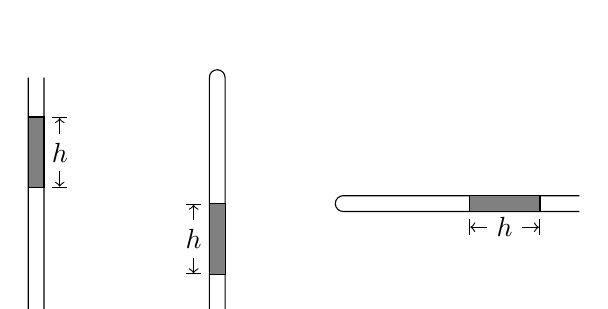
\begin{tikzpicture}
    
	\begin{scope}[]
		\draw[|<->|] (.4,1.6)--node[fill=white]{\(h\)}(.4,2.5);
		\draw (0,3)--(0,0) arc(-180:0:.1)--(.2,3);
		\draw[fill=gray] (0,1.6) rectangle(.2,2.5);
	\end{scope}
    \begin{scope}[xshift=2.5cm,yshift=3cm,rotate=180]
		\draw[|<->|] (.4,1.6)--node[fill=white]{\(h\)}(.4,2.5);
		\draw (0,3)--(0,0) arc(-180:0:.1)--(.2,3);
		\draw[fill=gray] (0,1.6) rectangle(.2,2.5);
	\end{scope}
    \begin{scope}[xshift=4cm,yshift=1.5cm,rotate=-90]
        \draw[|<->|] (.4,1.6)--node[fill=white]{\(h\)}(.4,2.5);
		\draw (0,3)--(0,0) arc(-180:0:.1)--(.2,3);
		\draw[fill=gray] (0,1.6) rectangle(.2,2.5);
	\end{scope}
\end{tikzpicture}
\hspace*{3em}
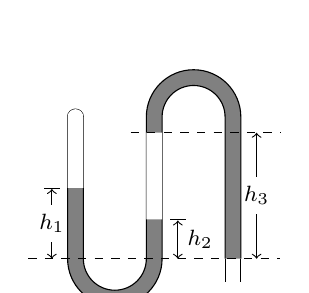
\begin{tikzpicture}[font=\footnotesize]
    \draw[|<->] (-.2,.9)--node[fill=white]{\(h_1\)}(-.2,0);
    \draw[|<->] (1.4,.5)--node[right]{\(h_2\)}(1.4,0);
    \draw[<->] (2.4,1.6)--node[fill=white]{\(h_3\)}(2.4,0);
    \draw[fill=gray] (2,0)--(2,1.8) arc(0:180:.4)--(1.2,0) arc(0:-180:.6)--(0,1.8) arc(180:0:.1)--(.2,0) arc(-180:0:.4)--(1,1.8) arc(180:0:.6)--(2.2,0);
    \fill[white] (0,.9)--(0,1.8)arc(180:0:.1)--(.2,.9)--(0,.9) (1,.5) rectangle(1.2,1.6);
    \draw (2,0)--(2,-.3) (2.2,0)--(2.2,-.3);
    \draw[dashed] (-.5,0)--(2.7,0) (.8,1.6)--(2.7,1.6);
\end{tikzpicture}
\vspace*{1.5cm}

\lsn{8}第一类永动机和第二类永动机为什么不可能存在？
\vspace*{2.5cm}

\lsn{9}如下图所示，将粗细不同的玻璃管插入水和水银中，试画出试管中的液面

\begin{tikzpicture}[font=\footnotesize]
    \draw[fill=gray!30] (0,0) rectangle(4,1.5);
    \draw[very thick] (0,3)--(0,0)--(4,0)--(4,3);
    \draw[fill=white,draw=white] (1.4,.5) rectangle(1.7,1.6) (2.5,.5) rectangle(2.65,1.6);
    \foreach \x in {1.4,1.7,2.5,2.65}
        \draw[very thin] (\x,.5)--(\x,2.8);
    \node at(3.5,.4){水};
    \begin{scope}[xshift=6cm]
        \draw[fill=gray!30] (0,0) rectangle(4,1.5);
        \draw[very thick] (0,3)--(0,0)--(4,0)--(4,3);
        \draw[fill=white,draw=white] (1.4,.5) rectangle(1.7,1.6) (2.5,.5) rectangle(2.65,1.6);
        \foreach \x in {1.4,1.7,2.5,2.65}
            \draw[very thin] (\x,.5)--(\x,2.8);
        \node at(3.5,.4){水银};
    \end{scope}
\end{tikzpicture}

\lsn{10}一只轮胎容积为\(V=\) \,\qty{10}{L}，已装有\(p_1 =\) \,\qty{1}{atm}的空气。现用打气筒给打气，已知打气筒的容积为\(V_0 =\) \,\qty{1}{L}，要使胎内气体压强达到\(p_2 =\) \,\qty{2.5}{atm}，应至少打多少次气？(设打气过程中轮胎容积及气体温度维持不变，大气压强\(p_0 =\) \,\qty{1}{atm})
\vspace*{2cm}

\lsn{11}在测油酸分子直径的实验中，如果使用长时间放置的酒精油酸溶液，测得的油酸分子直径会偏大还是偏小？为什么？

\newpage
\lsn{12}质量不变的理想气体经历\(a \to b \to c \to a\)的循环过程，其中\(a\to b\)是等温膨胀过程，\(b\to c\) 是等容过程，\(c\to a\)是等压过程，分别在\(p - V\)、\(p - T\)、\(V - T\)图像中画出该循环过程，并分析各个过程的\(\Delta U\)、\(W\)、\(Q\) 以及整个循环过程是吸热还是放热。

\begin{tikzpicture}[font=\footnotesize,>=latex]
    \draw[blue,->] (0,0)node[below left]{\(O\)}--(4,0) node[right]{\(V\)};
    \draw[blue,->] (0,0)--(0,3) node[above]{\(p\)};
\end{tikzpicture}
\vspace*{1cm}

\begin{tikzpicture}[font=\footnotesize,>=latex]
    \draw[blue,->] (0,0)node[below left]{\(O\)}--(4,0) node[right]{\(T\)};
    \draw[blue,->] (0,0)--(0,3) node[above]{\(p\)};
\end{tikzpicture}
\vspace*{1cm}

\begin{tikzpicture}[font=\footnotesize,>=latex]
    \draw[blue,->] (0,0)node[below left]{\(O\)}--(4,0) node[right]{\(T\)};
    \draw[blue,->] (0,0)--(0,3) node[above]{\(V\)};
\end{tikzpicture}
\end{document}
